\documentclass{article}
\usepackage{amsmath}
\usepackage{enumerate}
\usepackage{listings}
\usepackage{moreverb}
\usepackage[margin=1in]{geometry}
\usepackage{graphicx}
\usepackage{dsfont}
\title{STA 360: Lab 9}
\author{Michael Lin}

\begin{document}
\maketitle

\begin{enumerate}
\item See below for priors used and the resulting posterior distributions for $\mu$ and $\sigma^2$.

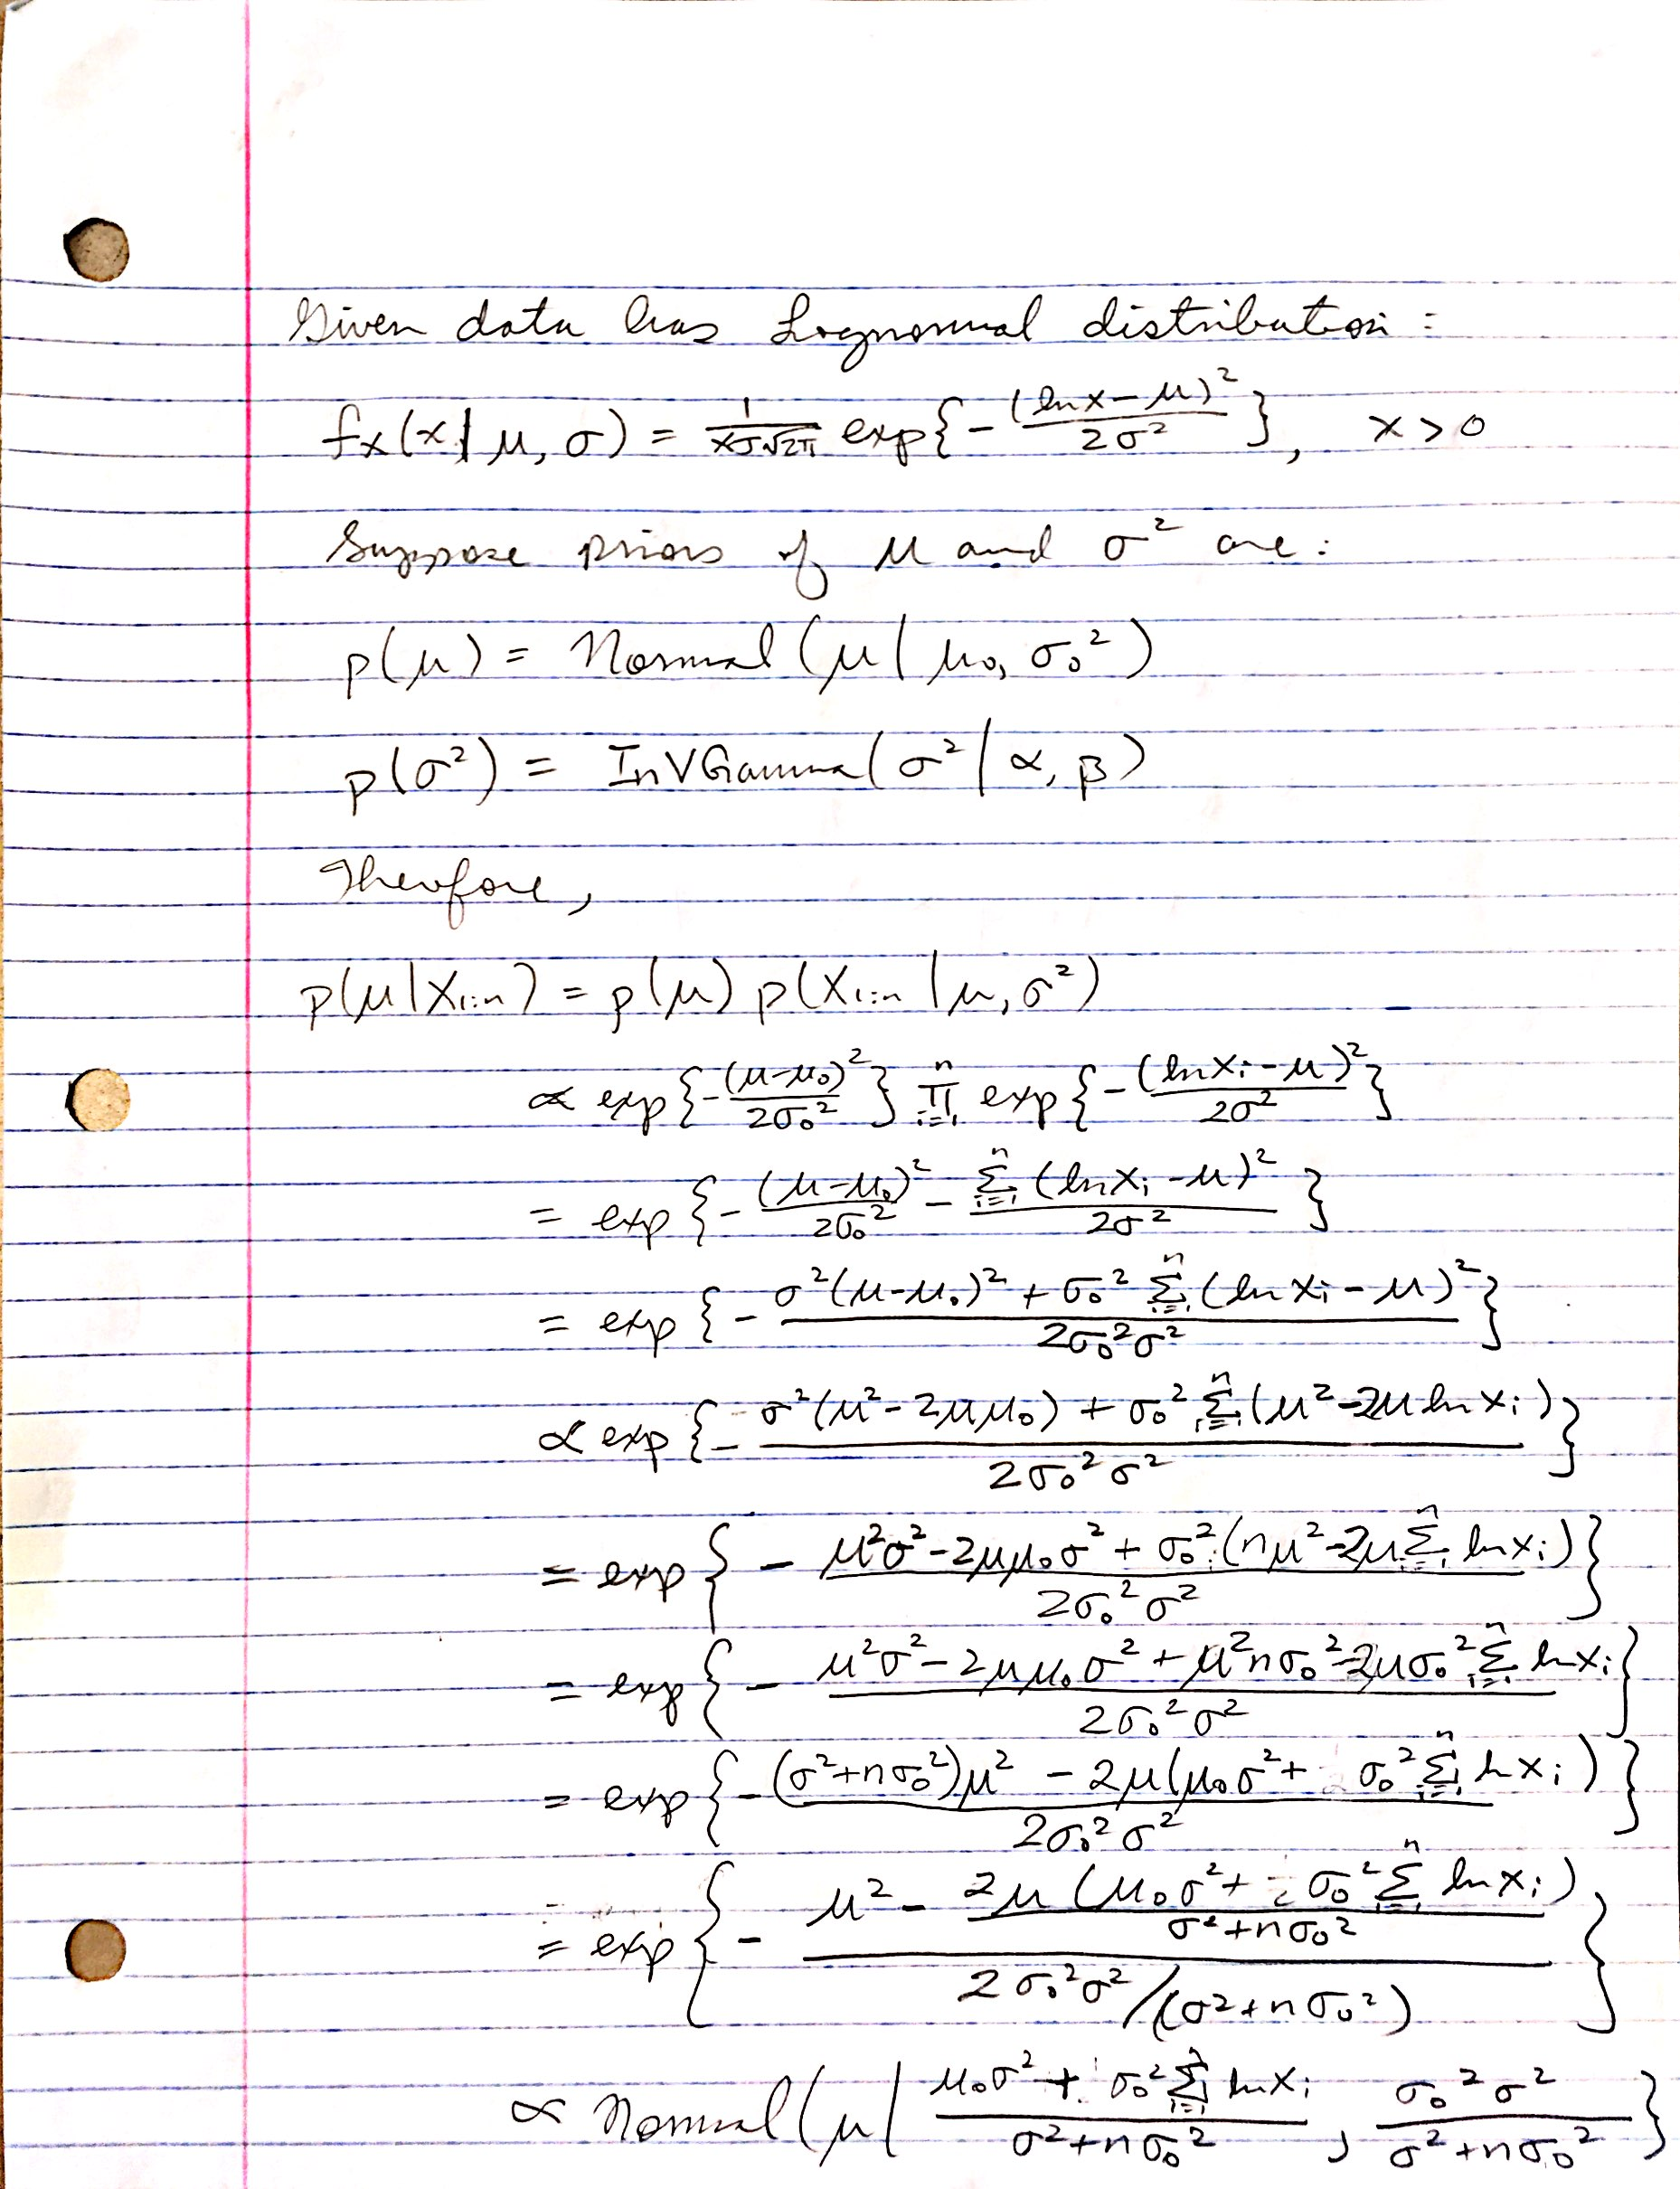
\includegraphics[scale = 0.2]{page1.jpg}\\
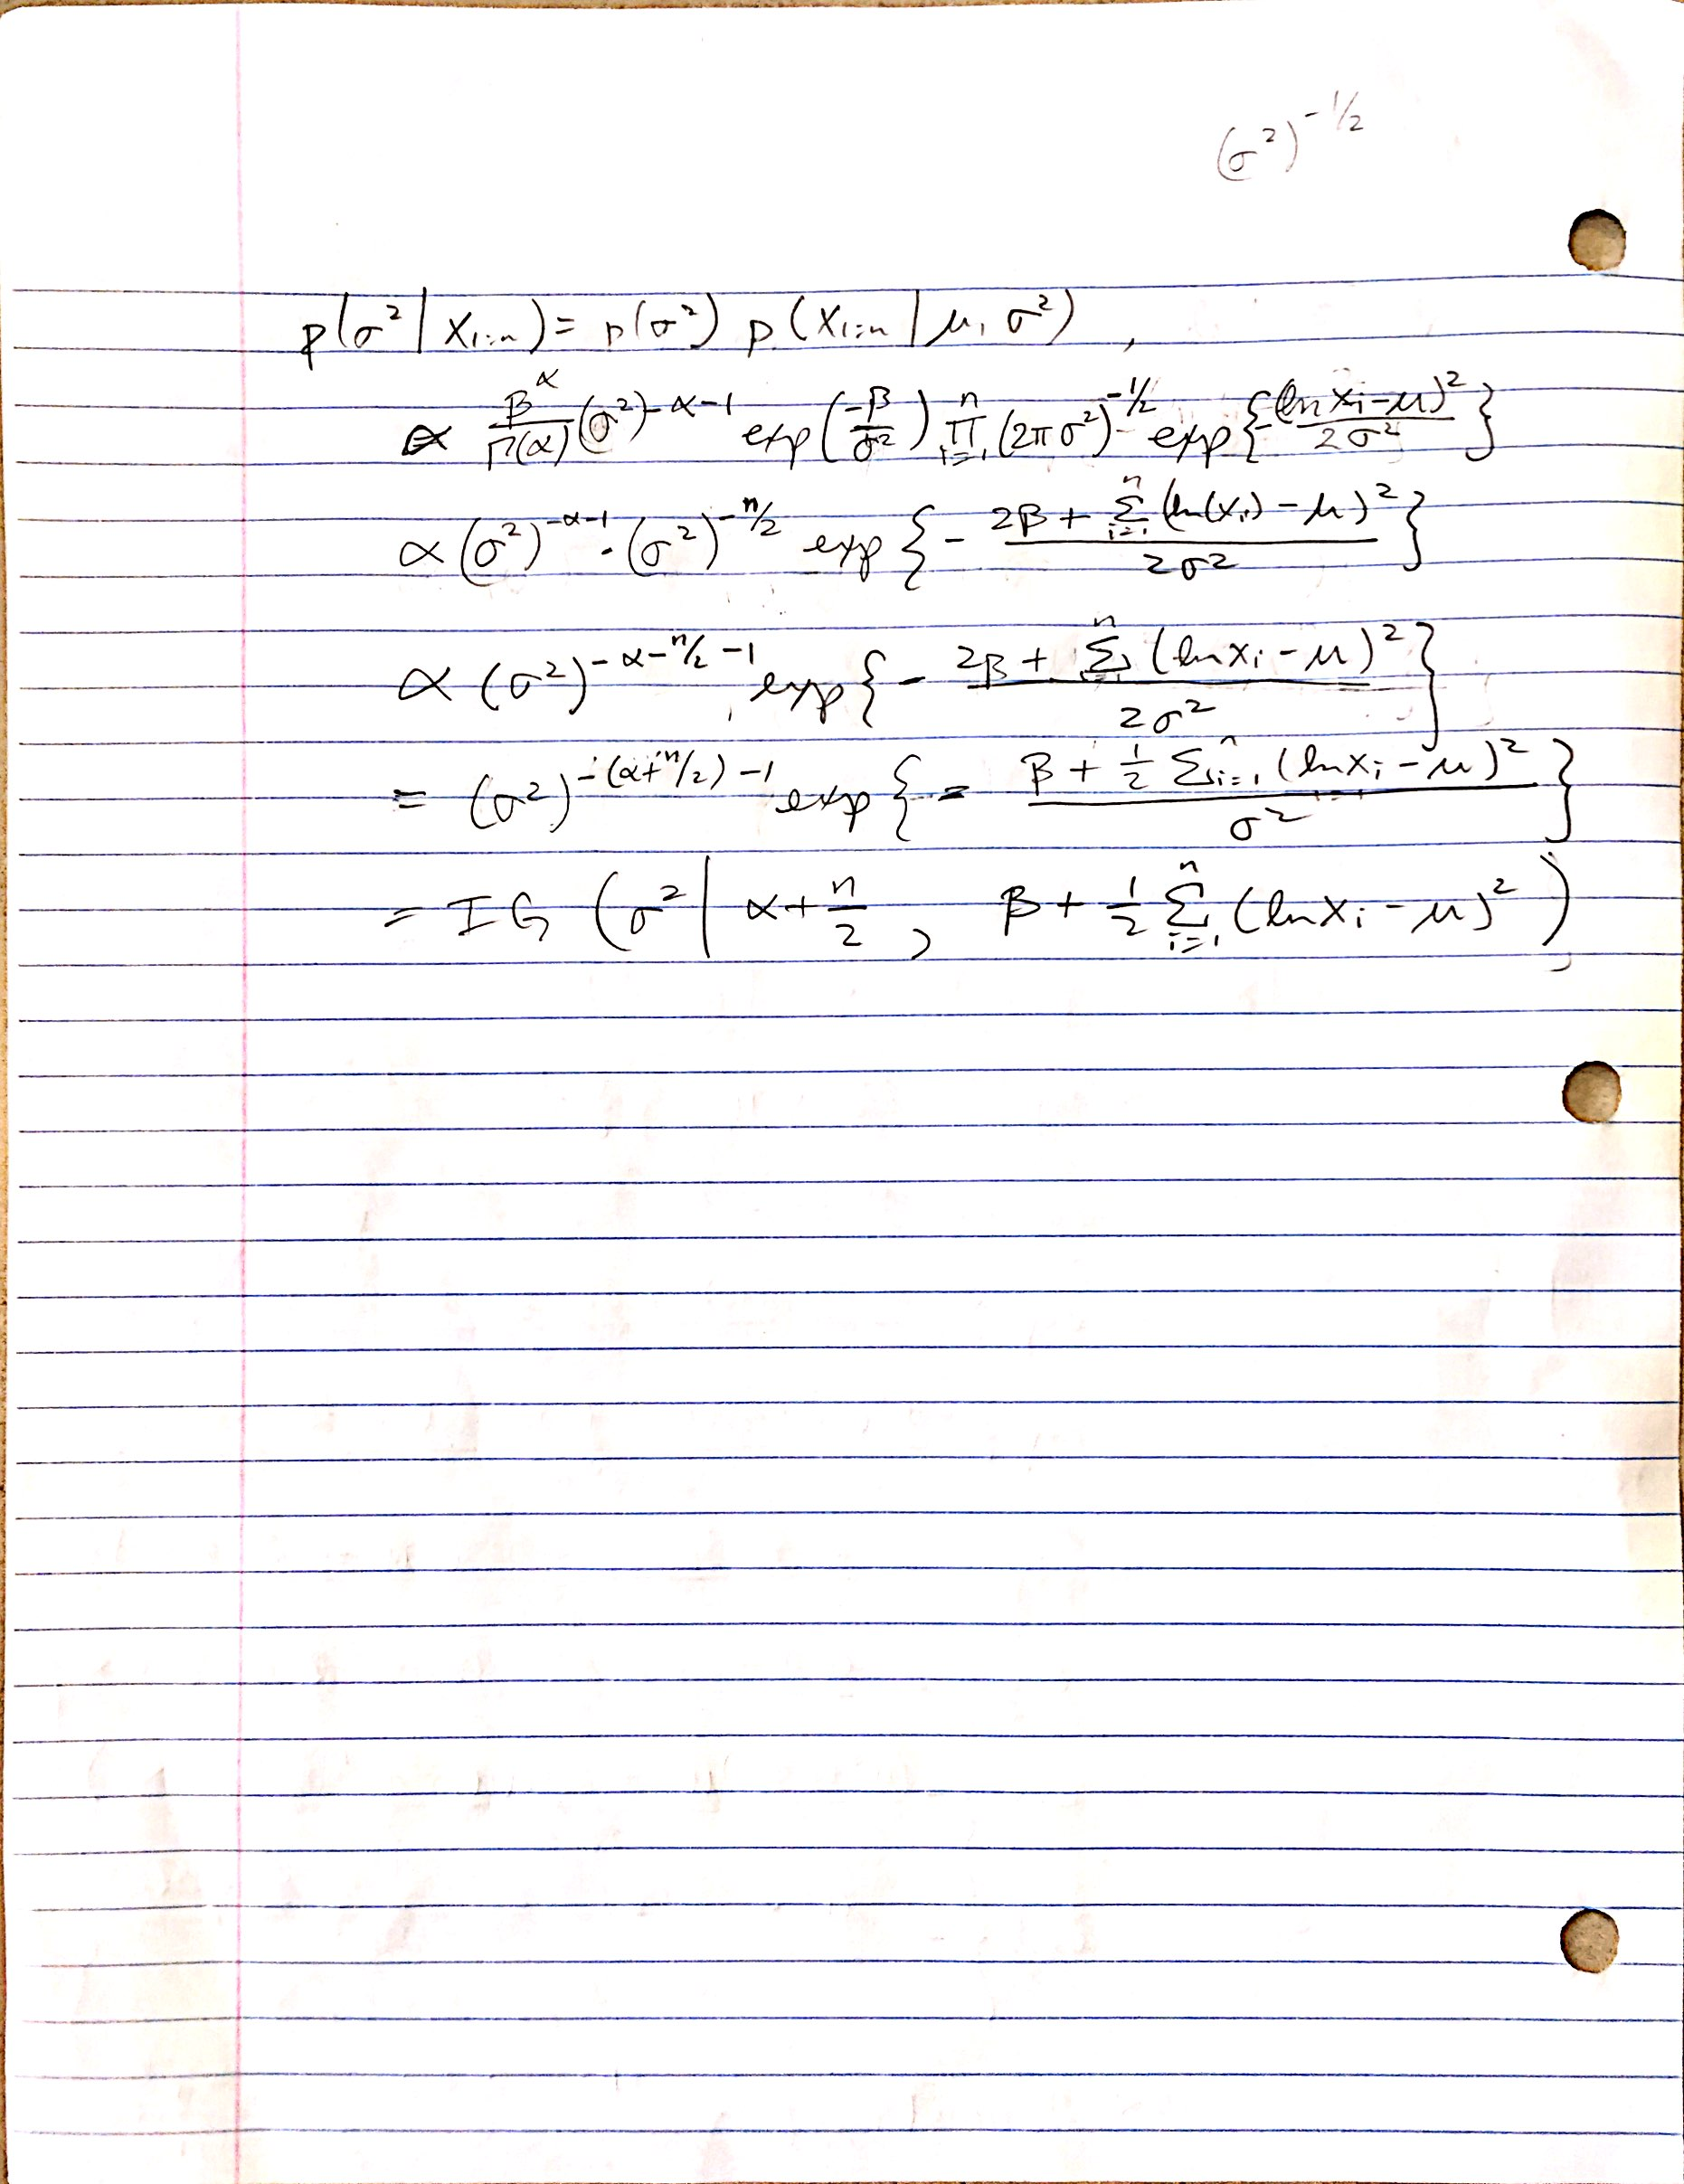
\includegraphics[scale = 0.2]{page2.jpg}

\pagebreak

\item See below for trace plots. We used $\alpha, \beta = 0$ for $\sigma^2$ because it's a Jeffery's prior. We also set $\mu_0=0$ and $\sigma_0^2=0$ to allow large prior variance (i.e. uninformative prior). The Gibbs sampler appears to have converged and explored the space reasonably well.

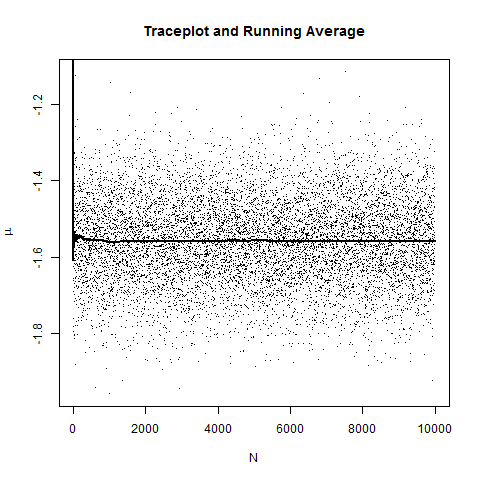
\includegraphics[scale = 0.4]{MUplot.png}
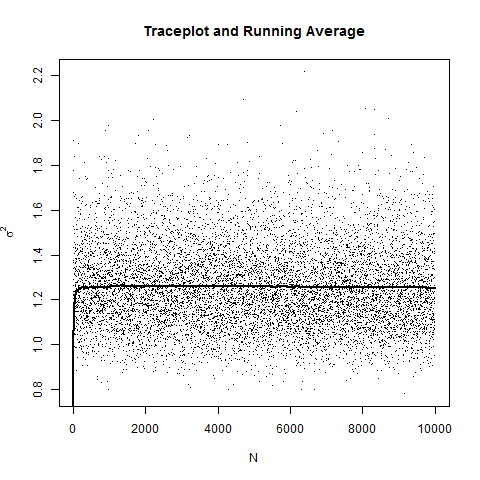
\includegraphics[scale = 0.4]{SIGplot.png}

\item See below for respective 95\% confidence interval.

$$ \text{CI}(\text{mean}) = [0.7066048, 0.1072423] $$

$$ \text{CI}(\text{variance}) = [0.1586194, 1.0671797] $$
\end{enumerate}

\pagebreak

See below for R code:

\listinginput[1]{1}{lab9.r}

\end{document}